\section{Introduction}\label{sec:intro}

intro



% ============================================================
% Introductory motivating example, DAG-centric.
% Two DAG sketches (before/after) with four numbered annotations.
% ============================================================

% Required packages (in main.tex):
%   \usepackage{tikz}
%   \usetikzlibrary{positioning, arrows.meta, fit, calc, backgrounds}
%   \usepackage{xcolor}  % for the textcolor in source labels

\usetikzlibrary{positioning, arrows.meta, fit, calc, backgrounds}

\begin{figure*}[t]
\centering

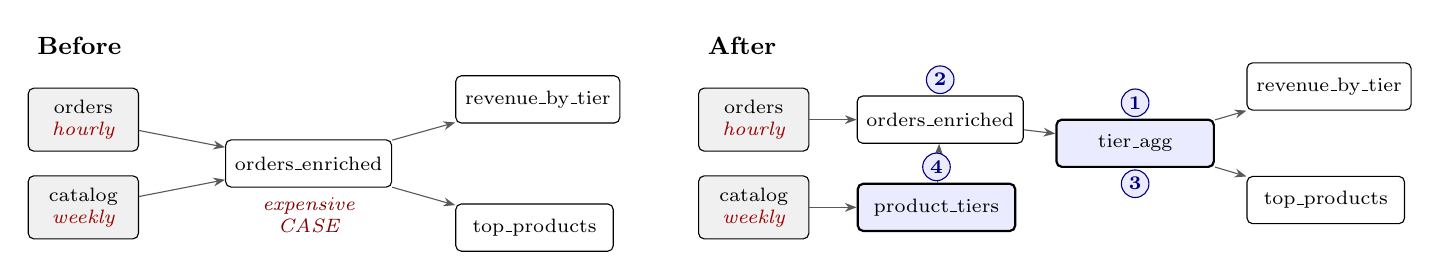
\begin{tikzpicture}[
  font=\small,
  node distance=5mm and 7mm,
  src/.style={draw, rounded corners=2pt, fill=gray!12,
              minimum width=14mm, minimum height=8mm,
              align=center, font=\scriptsize},
  model/.style={draw, rounded corners=2pt, fill=white,
                minimum width=20mm, minimum height=6mm,
                align=center, font=\scriptsize},
  newmodel/.style={draw, rounded corners=2pt, fill=blue!8, thick,
                   minimum width=20mm, minimum height=6mm,
                   align=center, font=\scriptsize},
  freq/.style={font=\scriptsize\itshape, color=red!60!black},
  edge/.style={-{Stealth[length=1.5mm]}, thin, gray!70!black},
  annot/.style={font=\scriptsize\bfseries, color=blue!50!black,
                draw=blue!50!black, circle, inner sep=0pt,
                minimum size=3.5mm, fill=blue!8},
]

% ------------------- BEFORE DAG (left half) -------------------
\node[font=\bfseries\small] (beforehdr) at (0,0) {Before};

\node[src, below=3mm of beforehdr.south west, anchor=north west] (orders0)
  {orders\\\textcolor{red!60!black}{\itshape hourly}};
\node[src, below=3mm of orders0] (catalog0)
  {catalog\\\textcolor{red!60!black}{\itshape weekly}};

\node[model, right=18mm of $(orders0)!0.5!(catalog0)$] (enr0) {orders\_enriched};
\node[model, above right=2mm and 8mm of enr0] (rev0) {revenue\_by\_tier};
\node[model, below right=2mm and 8mm of enr0] (top0) {top\_products};

\draw[edge] (orders0) -- (enr0);
\draw[edge] (catalog0) -- (enr0);
\draw[edge] (enr0) -- (rev0);
\draw[edge] (enr0) -- (top0);

% Callout: expensive CASE inside enr (motivates the moves)
\node[font=\scriptsize\itshape, color=red!50!black,
      below=0mm of enr0, align=center]
  {expensive\\CASE};

% ------------------- AFTER DAG (right half) -------------------
\node[font=\bfseries\small, right=72mm of beforehdr] (afterhdr) {After};

\node[src, below=3mm of afterhdr.south west, anchor=north west] (orders1)
  {orders\\\textcolor{red!60!black}{\itshape hourly}};
\node[src, below=3mm of orders1] (catalog1)
  {catalog\\\textcolor{red!60!black}{\itshape weekly}};

% New: product_tiers between catalog and enr (move 4)
\node[newmodel, right=6mm of catalog1] (ptiers1) {product\_tiers};

\node[model, right=6mm of orders1] (enr1) {orders\_enriched};

% New: tier_agg between enr and consumers (moves 1-3)
\node[newmodel, right=4mm of enr1, yshift=-3mm] (tagg1) {tier\_agg};

\node[model, above right=1mm and 4mm of tagg1] (rev1) {revenue\_by\_tier};
\node[model, below right=1mm and 4mm of tagg1] (top1) {top\_products};

\draw[edge] (orders1) -- (enr1);
\draw[edge] (catalog1) -- (ptiers1);
\draw[edge] (ptiers1) -- (enr1);
\draw[edge] (enr1) -- (tagg1);
\draw[edge] (tagg1) -- (rev1);
\draw[edge] (tagg1) -- (top1);

% --- Numbered annotations on the After DAG ---
% (1) factor: points at tier_agg
\node[annot] at ($(tagg1.north) + (0,2mm)$) (a1) {1};
% (2) drop columns: points at enr
\node[annot] at ($(enr1.north) + (0,2mm)$) (a2) {2};
% (3) materialization: points at tier_agg's interior
\node[annot] at ($(tagg1.south) + (0,-2mm)$) (a3) {3};
% (4) frequency split: points at product_tiers
\node[annot] at ($(ptiers1.north) + (0,2mm)$) (a4) {4};

\end{tikzpicture}

\vspace{2mm}

% --- Move legend below the DAGs ---
\begin{minipage}{0.97\textwidth}
\footnotesize
\begin{tabular}{@{}r@{\hspace{1.5mm}}p{0.92\textwidth}@{}}
\textbf{(1)} & \emph{Factor non-local shared work.} Both consumers group by \texttt{tier}; the optimizer extracts the shared aggregation into a new model invisible at any single SQL file. \\[0.5mm]
\textbf{(2)} & \emph{Equivalence is required at project outputs, not at every intermediate.} The optimizer can change an intermediate model in ways that no single-query rewriter would consider safe---e.g., narrowing its schema---as long as the project's leaf outputs are preserved. \\[0.5mm]
\textbf{(3)} & \emph{Refactoring and materialization are coupled.} The factorization in (1) is a win as a table and a wash as a view; refactoring decisions cannot be made without the materialization decision. \\[0.5mm]
\textbf{(4)} & \emph{Frequency is itself a structural dimension.} The expensive classification depends only on weekly data but lives inside an hourly model; splitting it onto the slow cadence requires a DAG rewrite invisible to per-execution cost. \\
\end{tabular}
\end{minipage}

\caption{An introductory walkthrough previewing the characteristics of dbt optimization addressed by \tool. The original DAG (\emph{Before}) has two sources at different update rates, an enriched intermediate, and two consumers; the whole pipeline runs hourly. \tool transforms it (\emph{After}) along four dimensions, summarized in the legend and addressed jointly in \S\ref{sec:approach}.}
\label{fig:intro-example}
\end{figure*}